\documentclass[11pt,aspectratio=169]{beamer}

% Theme
\usetheme{Madrid}
\usecolortheme{default}

% Packages
\usepackage{graphicx}
\usepackage{booktabs}
\usepackage{array}
\usepackage{hyperref}
\usepackage{tikz}
\usetikzlibrary{shapes,arrows,positioning,shadows}

% Title information
\title{Git, GitHub, and VS Code}
\subtitle{Agentic AI for Research: From One Task to Orchestration}
\author{Tomas Larroucau }
\institute{Arizona State University}
\date{Monday, October 26, 2026}

% Remove navigation symbols
\setbeamertemplate{navigation symbols}{}

% Footer
\setbeamertemplate{footline}[frame number]


% Small source notes; slide body remains at the original 11pt size.
\newcommand{\sources}[1]{{\scriptsize\color{gray}#1}}


\begin{document}

% Revision item 1; original frame: 1

\begin{frame}
\titlepage
\end{frame}

% Revision item 2; original frame: 3

\begin{frame}{Why This Workshop?}
\begin{columns}[t]
\begin{column}{0.48\textwidth}
\textbf{The Problem:}
\begin{itemize}
\item Research projects grow messy fast
\item Code, writing, and decisions drift apart
\item More agents can mean more work to supervise
\end{itemize}
\end{column}
\begin{column}{0.48\textwidth}
\textbf{What We Will Do:}
\begin{itemize}
\item Work in one research environment
\item Turn a task into a reviewable change
\item Coordinate agents with clear ownership
\end{itemize}
\end{column}
\end{columns}
\par\vspace{0.5cm}
\begin{block}{By the end}
You can give an agent a bounded task, inspect its changes, and decide whether the work is ready to share.
\end{block}
\end{frame}

% Revision item 3; original frame: 2

\begin{frame}{Our 90 Minutes}
\centering
\begin{tabular}{rl}
\toprule
\textbf{Minutes} & \textbf{What we do} \\
\midrule
0--7 & The research workflow and today's goal \\
7--18 & VS Code and the project template \\
18--31 & Git, issues, and a reviewable change \\
31--43 & Claude Code and Codex: ten useful comparisons \\
43--58 & Live demo: plan, edit, inspect, verify \\
58--68 & Short exercise or paired review \\
68--82 & Orchestration: tasks, sessions, worktrees, resources \\
82--90 & Questions and one next step \\
\bottomrule
\end{tabular}
\par\vspace{0.3cm}
\begin{block}{Keep moving}
If setup fails, follow the demonstration or work with a partner. The appendix is for later.
\end{block}
\end{frame}

% Revision item 4; original frame: 5

\begin{frame}{The Symbiosis: Agents as Builders}
\begin{columns}[c]
\begin{column}{0.37\textwidth}

\includegraphics[width=\columnwidth]{figures/Symbiosis.png}
\end{column}
\begin{column}{0.59\textwidth}
\begin{itemize}\setlength{\itemsep}{0.35cm}
\item \textbf{VS Code}: read, write, run, and review in the project
\item \textbf{Git and GitHub}: saved history and shared decisions
\item \textbf{Agents}: help build and check the workflow itself
\end{itemize}
\par\vspace{0.25cm}
The dinosaur can help build the fence. We still inspect the fence.
\end{column}
\end{columns}
\par\vspace{0.25cm}
\small Git can restore recorded files. It cannot retract a message, recover every unsaved file, or undo an external action.
\end{frame}

% Revision item 5; original frame: 10

\begin{frame}{VS Code: An Integrated Research Environment}
\begin{columns}[t]
\begin{column}{0.48\textwidth}
\textbf{Read and Write}
\begin{itemize}
\item Browse papers, notes, and project files
\item Edit LaTeX and Markdown
\item Preview a PDF beside its source
\item Search the whole project
\end{itemize}
\end{column}
\begin{column}{0.48\textwidth}
\textbf{Run and Collaborate}
\begin{itemize}
\item Run scripts in the terminal
\item Inspect Git diffs and history
\item Work with issues and pull requests
\item Use agent extensions or CLI sessions
\end{itemize}
\end{column}
\end{columns}
\par\vspace{0.4cm}
\textbf{Demo:} Open the project folder. Read the README, preview the slides, inspect a diff, and open an agent session.
\par\vspace{0.3cm}
\small PDF, language, and agent features depend on the extensions you install. Start with what your project needs.
\end{frame}

% Revision item 6; original frame: 7

\begin{frame}{Reproducible Research Template}
\hypertarget{main-project-structure}{}
\begin{columns}[t]
\begin{column}{0.50\textwidth}
\begin{itemize}
\item \texttt{data/raw/}: teaching data, kept unchanged
\item \texttt{scripts/}: processing and analysis
\item \texttt{output/}: generated figures and tables
\item \texttt{tex/}: paper and Beamer sources
\end{itemize}
\end{column}
\begin{column}{0.46\textwidth}
\begin{itemize}
\item \texttt{Makefile}: build steps
\item \texttt{README.md}: how to use the project
\item \texttt{AGENTS.md}: project guidance
\item \texttt{.gitignore}: untracked files to exclude
\end{itemize}
\end{column}
\end{columns}
\par\vspace{0.4cm}
\textbf{Key Principle:} Generate research outputs from scripts. Review source edits and record the decisions behind them.
\par\vspace{0.25cm}
\small Template: \url{https://github.com/tlarroucau/AI_workshop}
\par\vspace{0.2cm}
\hyperlink{appendix-makefile}{\beamerbutton{Build commands in the appendix}}
\end{frame}

% Revision item 7; original frame: 8

\begin{frame}{Workshop Prerequisites}
\begin{columns}[t]
\begin{column}{0.48\textwidth}
\textbf{Follow and Review}
\begin{itemize}
\item A browser and the workshop materials
\item VS Code and Git for the local exercise
\item A local copy of the template
\item A partner if setup is incomplete
\end{itemize}
\end{column}
\begin{column}{0.48\textwidth}
\textbf{Run an Agent Yourself}
\begin{itemize}
\item One supported agent, signed in
\item Check your account's access and limits
\item GitHub account for hosted collaboration
\item Python and LaTeX only for full builds
\end{itemize}
\end{column}
\end{columns}
\par\vspace{0.35cm}
\begin{block}{Today's exercise}
A README edit works without Python, LaTeX, or an MCP server. Claude Code and Codex are demonstrated; you do not need both subscriptions.
\end{block}
\end{frame}

% Revision item 8; original frame: 22

\begin{frame}[fragile]{Git Core Concepts}
\begin{enumerate}
    \item \textbf{Repository (repo)}: Project folder tracked by Git
    
    \item \textbf{Commit}: Snapshot of the changes you staged
    
    \item \textbf{Branch}: Parallel version of your repository
    
    \item \textbf{Merge}: Combine changes from different branches
    
    \item \textbf{Remote}: Another repository (often hosted on GitHub)
\end{enumerate}

\par\vspace{0.3cm}

\begin{block}{Basic Workflow}
\begin{verbatim}
git add file.py          # Stage changes
git commit -m "message"  # Save snapshot
git push                 # Upload to remote
\end{verbatim}
\end{block}
\end{frame}

% Revision item 9; original frame: 23

\begin{frame}{The Git Workflow}
\begin{center}
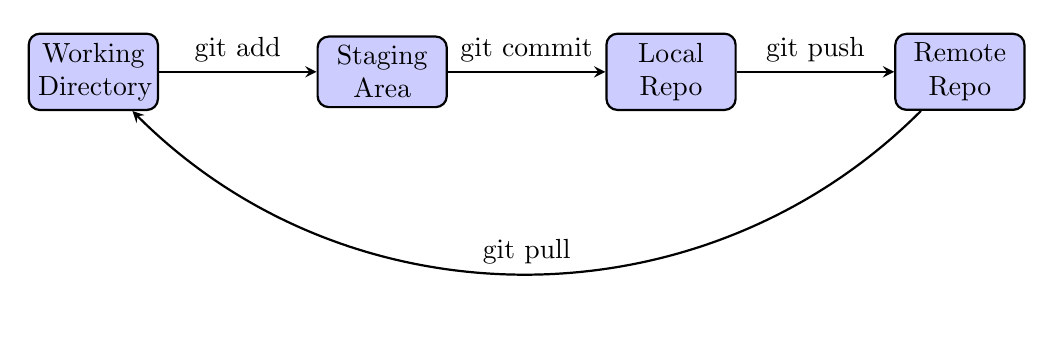
\begin{tikzpicture}[node distance=2cm, auto, thick]
    \tikzstyle{box} = [rectangle, draw, fill=blue!20, text width=4em, text centered, rounded corners, minimum height=2em]
    \tikzstyle{arrow} = [->, >=stealth]
    
    \node [box] (working) {Working\\Directory};
    \node [box, right=of working] (staging) {Staging\\Area};
    \node [box, right=of staging] (local) {Local\\Repo};
    \node [box, right=of local] (remote) {Remote\\Repo};
    
    \draw [arrow] (working) -- node {git add} (staging);
    \draw [arrow] (staging) -- node {git commit} (local);
    \draw [arrow] (local) -- node {git push} (remote);
    \draw [arrow] (remote) to [bend left=45] node[above] {git pull} (working);
\end{tikzpicture}
\end{center}

\par\vspace{0.3cm}
\begin{itemize}
    \item Edit files in working directory
    \item Stage changes you want to commit
    \item Commit records the staged changes in local history
    \item Push shares with collaborators
\end{itemize}
\end{frame}

% Revision item 10; original frame: 33

\begin{frame}{GitHub Issues: Shared Research Context}
\begin{columns}[t]
\begin{column}{0.48\textwidth}
\textbf{An issue records the task}
\begin{itemize}
\item Research goal and why it matters
\item Relevant files and decisions
\item Owner and allowed scope
\item Evidence required to finish
\end{itemize}
\end{column}
\begin{column}{0.48\textwidth}
\begin{block}{Example: clarify the Quick Start}
Separate a README-only exercise from a full analysis build. Verify every listed command against the Makefile. Keep analysis and data unchanged.
\end{block}
\end{column}
\end{columns}
\par\vspace{0.4cm}
Coauthors can read the issue after the chat ends. Ask each new session to read it and report what remains unresolved.
\par\vspace{0.2cm}
\small The example is a task brief. Creating or updating a hosted issue requires the appropriate access and authorization.
\end{frame}

% Revision item 11; original frame: 35

\begin{frame}{GitHub Workflow: Pull Requests}
\textbf{What are Pull Requests (PRs)?}
\begin{itemize}
    \item Propose changes to repository
    \item Enable code review before merging
    \item Discuss implementation details
\end{itemize}

\par\vspace{0.1cm}

\textbf{PR Workflow:}

\begin{center}
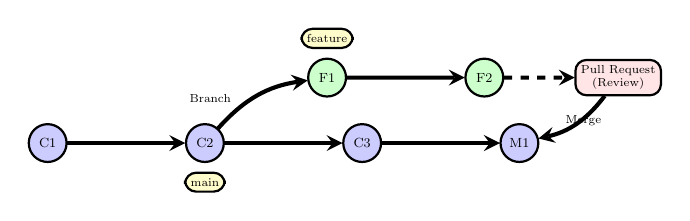
\begin{tikzpicture}[scale=0.6, transform shape, node distance=2.5cm, auto, thick]
    \tikzstyle{commit} = [circle, draw, fill=blue!20, minimum size=0.8cm, font=\footnotesize]
    \tikzstyle{commit_feature} = [circle, draw, fill=green!20, minimum size=0.8cm, font=\footnotesize]
    \tikzstyle{arrow} = [->, >=stealth, line width=1.5pt]
    \tikzstyle{label_box} = [rectangle, draw, fill=yellow!20, rounded corners, font=\scriptsize]
    \tikzstyle{pr_box} = [rectangle, draw, fill=red!10, rounded corners, font=\scriptsize, align=center]

    \node [commit] (c1) {C1};
    \node [commit, right=of c1] (c2) {C2};
    \node [commit, right=of c2] (c3) {C3};
    \node [commit, right=of c3] (m1) {M1};
    
    \node [commit_feature, above right=0.8cm and 2cm of c2] (f1) {F1};
    \node [commit_feature, right=of f1] (f2) {F2};
    
    \draw [arrow] (c1) -- (c2);
    \draw [arrow] (c2) -- (c3);
    \draw [arrow] (c3) -- (m1);
    
    \draw [arrow] (f1) -- (f2);
    
    \draw [arrow] (c2) to [bend left=20] node[near start, above left, font=\scriptsize] {Branch} (f1);
    
    \node [pr_box, right=1.5cm of f2] (pr) {Pull Request\\(Review)};
    \draw [arrow, dashed] (f2) -- (pr);
    \draw [arrow] (pr) to [bend left=20] node[near end, above right, font=\scriptsize] {Merge} (m1);
    
    \node [label_box, below=0.2cm of c2] {main};
    \node [label_box, above=0.2cm of f1] {feature};
    
\end{tikzpicture}
\end{center}

\par\vspace{-0.3cm}
\begin{columns}[t]
    \begin{column}{0.5\textwidth}
        \footnotesize
        \begin{enumerate}
            \item Create and push feature branch
            \item Open Pull Request on GitHub
        \end{enumerate}
    \end{column}
    \begin{column}{0.5\textwidth}
        \footnotesize
        \begin{enumerate}
            \setcounter{enumi}{2}
            \item Review, discuss, and fix
            \item Merge when approved
        \end{enumerate}
    \end{column}
\end{columns}

\par\vspace{0.3cm}
\textbf{Review:} Does the diff satisfy the issue? What evidence supports merging?
\end{frame}

% Revision item 12; original frame: 15

\begin{frame}{What Is Agentic AI?}
\begin{center}
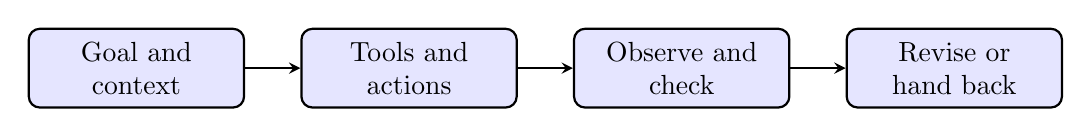
\begin{tikzpicture}[node distance=0.7cm,>=stealth,thick]
\tikzstyle{box}=[draw,rounded corners,fill=blue!10,text width=2.5cm,align=center,minimum height=1cm]
\node[box] (goal) {Goal and\\context};
\node[box,right=of goal] (act) {Tools and\\actions};
\node[box,right=of act] (check) {Observe and\\check};
\node[box,right=of check] (rev) {Revise or\\hand back};
\draw[->] (goal)--(act);\draw[->] (act)--(check);\draw[->] (check)--(rev);
\end{tikzpicture}
\end{center}
\par\vspace{0.35cm}
\begin{itemize}\setlength{\itemsep}{0.2cm}
\item An agent can read files, edit, run commands, and use connected tools when permitted.
\item The model, its tools, context, and permissions jointly determine what it can do.
\item Completion is a claim to check against the requested output and evidence.
\end{itemize}
\end{frame}

% Revision item 13; original frame: new

\begin{frame}{Model, Agent, and Interface}
\begin{block}{Three different choices}
\textbf{Model}: the system generating responses.\\[0.12cm]
\textbf{Agent harness}: instructions, tools, permissions, and execution loop.\\[0.12cm]
\textbf{Interface}: terminal, editor, desktop app, or web session.
\end{block}
\par\vspace{0.3cm}
Choosing a Claude model inside Copilot still uses Copilot's agent harness. It does not turn that session into Claude Code.
\par\vspace{0.3cm}
\textbf{Compare workflows on the same task:} context used, control of edits, review quality, time, and allowance consumed.
\par\vfill
\sources{\href{https://code.visualstudio.com/docs/agents/run/agent-harnesses}{VS Code: agent harnesses}}
\end{frame}

% Revision item 14; original frame: new

% Official-source comparison, checked October 25, 2026.
% URLs and detailed qualifications are recorded in workshop_review/source_notes.md.
\begin{frame}{Claude Code and Codex: Context and Planning}
\small
\renewcommand{\arraystretch}{1.22}
\begin{tabular}{>{\raggedright\arraybackslash}p{2.35cm}>{\raggedright\arraybackslash}p{5.1cm}>{\raggedright\arraybackslash}p{5.1cm}}
\toprule
\textbf{Feature / use} & \textbf{Claude Code} & \textbf{Codex} \\
\midrule
\textbf{1. Instructions} \newline Project conventions & \texttt{CLAUDE.md}; can import \texttt{@AGENTS.md}. Recent versions also support an \texttt{AGENTS.md} fallback. & \texttt{AGENTS.md}, including guidance scoped to subdirectories. \\
\textbf{2. Skills} \newline Repeat a workflow & \texttt{SKILL.md} in \texttt{.claude/skills/}; invoke the named skill. & \texttt{SKILL.md} in \texttt{.agents/skills/}; use \texttt{/skills} or \texttt{\$name}. \\
\textbf{3. Plan first} \newline Discuss before editing & \texttt{--permission-mode plan} or Shift+Tab. & \texttt{/plan} in supported sessions; read-only permissions add an explicit edit boundary. \\
\bottomrule
\end{tabular}
\par\vspace{0.25cm}
\normalsize
\textbf{Research use:} store project conventions once; make a table-audit skill; agree the scope of a revision before editing.
\par\vfill
\sources{\href{https://code.claude.com/docs/en/memory}{Claude instructions}, \href{https://code.claude.com/docs/en/skills}{skills}, \href{https://code.claude.com/docs/en/common-workflows}{planning}; \href{https://learn.chatgpt.com/docs/agent-configuration/agents-md}{Codex instructions}, \href{https://learn.chatgpt.com/docs/build-skills}{skills}, \href{https://learn.chatgpt.com/docs/learn/best-practices}{planning}.}
\end{frame}

\begin{frame}{Claude Code and Codex: Output, Tools, Control}
\small
\renewcommand{\arraystretch}{1.22}
\begin{tabular}{>{\raggedright\arraybackslash}p{2.35cm}>{\raggedright\arraybackslash}p{5.1cm}>{\raggedright\arraybackslash}p{5.1cm}}
\toprule
\textbf{Feature / use} & \textbf{Claude Code} & \textbf{Codex} \\
\midrule
\textbf{4. Output style} \newline Match the audience & Named styles; try \texttt{/output-style explanatory} while learning. & Instructions and \texttt{/personality} where supported; these are not identical to Claude's style system. \\
\textbf{5. Tools / MCP} \newline Connect the workflow & Built-in tools plus configured MCP servers. & Built-in tools plus configured MCP servers. \\
\textbf{6. Permissions} \newline Bound the actions & Permission modes and shell sandboxing are separate controls. & Approval policy and sandbox settings are separate controls. \\
\bottomrule
\end{tabular}
\par\vspace{0.25cm}
\normalsize
\textbf{Research use:} request a short instructor explanation, connect only needed tools, and inspect what can read, edit, execute, or send data.
\par\vfill
\sources{\href{https://code.claude.com/docs/en/output-styles}{Claude styles}, \href{https://code.claude.com/docs/en/mcp}{MCP}, \href{https://code.claude.com/docs/en/permissions}{permissions}; \href{https://learn.chatgpt.com/docs/developer-commands}{Codex commands}, \href{https://learn.chatgpt.com/docs/extend/mcp}{MCP}, \href{https://learn.chatgpt.com/docs/agent-approvals-security}{security}.}
\end{frame}

\begin{frame}{Claude Code and Codex: Sessions and Remote Work}
\small
\renewcommand{\arraystretch}{1.3}
\begin{tabular}{>{\raggedright\arraybackslash}p{2.35cm}>{\raggedright\arraybackslash}p{5.1cm}>{\raggedright\arraybackslash}p{5.1cm}}
\toprule
\textbf{Feature / use} & \textbf{Claude Code} & \textbf{Codex} \\
\midrule
\textbf{7. Sessions} \newline Resume a task & \texttt{--continue}, \texttt{--resume}, or \texttt{/resume}. & \texttt{codex resume}; \texttt{/compact} manages long context. Naming and forks depend on the surface. \\
\textbf{8. Remote control} \newline Supervise work elsewhere & Remote Control connects to a session on a running host. Eligibility and admin settings apply. & Remote connections are surface-dependent. CLI remote control is experimental; check the installed version. \\
\bottomrule
\end{tabular}
\par\vspace{0.35cm}
\normalsize
Save research decisions in files or issues. A resumed chat is useful context, but collaborators need a durable record.
\par\vspace{0.2cm}
\small Remote control is a view into work on another host, not automatic migration to cloud execution. Rehearse this optional demo in advance.
\par\vfill
\sources{\href{https://code.claude.com/docs/en/sessions}{Claude sessions}, \href{https://code.claude.com/docs/en/remote-control}{remote control}; \href{https://learn.chatgpt.com/docs/developer-commands}{Codex commands}, \href{https://learn.chatgpt.com/docs/remote-connections}{remote connections}.}
\end{frame}

\begin{frame}{Claude Code and Codex: Delegation and Review}
\small
\renewcommand{\arraystretch}{1.3}
\begin{tabular}{>{\raggedright\arraybackslash}p{2.35cm}>{\raggedright\arraybackslash}p{5.1cm}>{\raggedright\arraybackslash}p{5.1cm}}
\toprule
\textbf{Feature / use} & \textbf{Claude Code} & \textbf{Codex} \\
\midrule
\textbf{9. Delegation} \newline Separate bounded tasks & Subagents use separate contexts. \texttt{--worktree NAME} isolates a working directory. & Subagents and Git worktree workflows are supported; setup depends on the surface. \\
\textbf{10. Review} \newline Challenge the change & Ask a separate session or reviewer agent to inspect the task, diff, and checks. & \texttt{/review}; connected GitHub review is a separate integration. \\
\bottomrule
\end{tabular}
\par\vspace{0.3cm}
\normalsize
\textbf{Research use:} one agent drafts, another checks sources, and a reviewer looks for mistakes. Assign each writer distinct files or a worktree.
\par\vspace{0.2cm}
\small Claude's experimental \texttt{/advisor} consults another model; it is different from Plan Mode. Availability and extra usage depend on provider and billing.
\par\vfill
\sources{\href{https://code.claude.com/docs/en/sub-agents}{Claude subagents}, \href{https://code.claude.com/docs/en/advisor}{advisor}; \href{https://learn.chatgpt.com/docs/agent-configuration/subagents}{Codex subagents}, \href{https://learn.chatgpt.com/docs/environments/git-worktrees}{worktrees}, \href{https://learn.chatgpt.com/docs/third-party/github}{review}.}
\end{frame}


% Revision item 15; original frame: 39

\begin{frame}{Live Demo: One Task, Visible Evidence}
\textbf{Task:} Make the README's Quick Start match how the repository actually builds.
\par\vspace{0.25cm}
\begin{enumerate}\setlength{\itemsep}{0.14cm}
\item Trace one existing paper table to its source; read the task brief and Makefile.
\item Ask for a plan. State scope and the acceptance criteria.
\item Make the edit in an isolated branch or output copy.
\item Read the diff and check the commands against the project.
\item Ask an independent session to find errors or omissions.
\item Show a prepared issue/PR example and explain verified closeout.
\end{enumerate}
\par\vspace{0.25cm}
\small Fallback: use the prepared before/after diff if authentication or the live agent stalls. We can inspect a complete change without waiting for a long run.
\end{frame}

% Revision item 16; original frame: new

\begin{frame}{A Prompt You Can Inspect}
\begin{block}{Plan first}
Read README.md, AGENTS.md, and Makefile. Explain how someone can do a documentation exercise and how they can run a full build. List inconsistencies and propose the smallest README edit. Do not change files yet.
\end{block}
\begin{block}{Then implement the agreed scope}
Edit README.md only. Keep research code and data unchanged. Verify each command against the repository. Return the diff, checks you actually performed, and unresolved questions. Stop before any push or hosted action.
\end{block}
\par\vspace{0.2cm}
\small A prompt expresses intent. Permission settings and a bounded workspace provide additional control.
\end{frame}

% Revision item 17; original frame: new

\begin{frame}{Ten-Minute Exercise: Review a Change}
\begin{enumerate}\setlength{\itemsep}{0.25cm}
\item \textbf{2 minutes}: Read the task and define what a correct result must include.
\item \textbf{4 minutes}: Ask one agent for a README edit, or inspect the prepared diff with a partner.
\item \textbf{3 minutes}: Find one claim to verify. Compare it with the Makefile or source file.
\item \textbf{1 minute}: Report: ready, needs changes, or blocked. Give one reason.
\end{enumerate}
\par\vspace{0.3cm}
\begin{block}{Success}
You can explain what changed, what was checked, and what still needs a human decision.
\end{block}
\end{frame}

% Revision item 18; original frame: new

\begin{frame}{You Choose the Level of Engagement}
\centering
\begin{tabular}{>{\raggedright\arraybackslash}p{3.4cm}>{\raggedright\arraybackslash}p{9.3cm}}
\toprule
\textbf{You specify} & \textbf{What the agent can help produce} \\
\midrule
Research question & Alternatives, assumptions, evidence to collect \\[0.15cm]
Project design & Task breakdown, dependencies, risks, acceptance criteria \\[0.15cm]
Bounded task & A proposed change and evidence that it works \\[0.15cm]
Exact implementation & Specific edits, commands, or code you want executed \\
\bottomrule
\end{tabular}
\par\vspace{0.4cm}
Move between levels as needed. Keep ownership of research choices and the decision to accept or share results.
\end{frame}

% Revision item 19; original frame: new

\begin{frame}{Parallel Work Needs Distinct Ownership}
\small
\begin{tabular}{>{\raggedright\arraybackslash}p{2.4cm}>{\raggedright\arraybackslash}p{3.8cm}>{\raggedright\arraybackslash}p{3.3cm}>{\raggedright\arraybackslash}p{2.4cm}}
\toprule
\textbf{Session} & \textbf{Task and output} & \textbf{Scope} & \textbf{Status} \\
\midrule
Planner & Agree scope and task brief & Read-only & Ready \\[0.18cm]
Claude Code A & Draft Quick Start edit & README; worktree A & Working \\[0.18cm]
Codex B & Check build instructions & Read-only; findings & Working \\[0.18cm]
Reviewer C & Review candidate diff & Read-only; findings & Waiting for A \\
\bottomrule
\end{tabular}
\par\vspace{0.35cm}
\normalsize
Each task has one owner, a defined input, an expected output, and a stop condition. The labels here are an example, not a model ranking.
\par\vspace{0.25cm}
\textbf{Control:} Inspect progress, interrupt, narrow scope, or reassign. Parallelize independent work; review follows a candidate change.
\end{frame}

% Revision item 20; original frame: new

\begin{frame}{One Machine: Clearly Labeled Sessions}
\begin{columns}[t]
\begin{column}{0.48\textwidth}
\textbf{A simple setup}
\begin{itemize}
\item Open separate terminal or editor sessions
\item Label provider, task, and working folder
\item Keep one shared task brief or board
\item Give each writer an isolated worktree
\end{itemize}
\end{column}
\begin{column}{0.48\textwidth}
\textbf{Optional shared view}
\begin{itemize}
\item VS Code documents discovery of local external Claude Code and Codex sessions
\item Enable the sessions list's \textit{External} filter
\item Check provider support before continuing a session
\end{itemize}
\end{column}
\end{columns}
\par\vspace{0.25cm}
\small Independent labeled sessions are enough. Local session discovery does not establish discovery of remote SSH or tmux sessions.
\par\vfill
\sources{\href{https://code.visualstudio.com/docs/agents/run/sessions/manage-sessions}{VS Code: manage sessions}. Codex continuation has a single-writer requirement; see appendix.}
\end{frame}

% Revision item 21; original frame: new

\begin{frame}{Separate Worktrees for Separate Writers}
\begin{columns}[t]
\begin{column}{0.48\textwidth}
\textbf{Branch}
\begin{itemize}
\item A line of Git history
\item Switching branches changes the current checkout
\end{itemize}
\end{column}
\begin{column}{0.48\textwidth}
\textbf{Worktree}
\begin{itemize}
\item A separate working directory
\item Lets writers use different branches at once
\end{itemize}
\end{column}
\end{columns}
\par\vspace{0.3cm}
\begin{block}{Coordination still matters}
Agree which files each agent owns. Keep outputs separate, review overlapping edits, and integrate one change at a time. Worktrees isolate files; they do not isolate shared databases or external services.
\end{block}
\small Commands are in the appendix. Start from an agreed commit and preserve existing work before branching.
\end{frame}

% Revision item 22; original frame: new

\begin{frame}{The Orchestrator Keeps the Big Picture}
\begin{columns}[t]
\begin{column}{0.48\textwidth}
\textbf{Personal assistant / orchestrator}
\begin{itemize}
\item Research goals and project priorities
\item Decisions, dependencies, and open questions
\item Task board and resource allocation
\item Reports back in terms of outcomes
\end{itemize}
\end{column}
\begin{column}{0.48\textwidth}
\textbf{Implementation sessions}
\begin{itemize}
\item A bounded task and local instructions
\item Relevant files and tools
\item Changes, checks, and evidence
\item A concise handoff when done or blocked
\end{itemize}
\end{column}
\end{columns}
\par\vspace{0.35cm}
Record the shared decisions outside an implementation-heavy terminal chat. Give collaborators the issue, candidate diff, and verification evidence.
\end{frame}

% Revision item 23; original frame: new

\begin{frame}{Several Projects and Machines}
\begin{center}
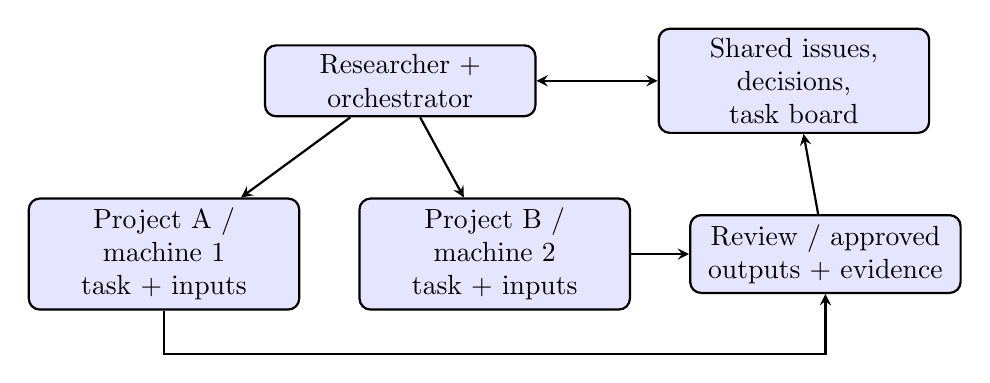
\begin{tikzpicture}[>=stealth,thick]
\tikzstyle{box}=[draw,rounded corners,fill=blue!10,align=center,minimum height=0.9cm,text width=3.2cm]
\node[box] (human) at (0,2.1) {Researcher +\\orchestrator};
\node[box] (board) at (5,2.1) {Shared issues,\\decisions, task board};
\node[box] (a) at (-3,-0.1) {Project A / machine 1\\task + inputs};
\node[box] (b) at (1.2,-0.1) {Project B / machine 2\\task + inputs};
\node[box] (c) at (5.4,-0.1) {Review / approved\\outputs + evidence};
\draw[<->] (human)--(board);
\draw[->] (human)--(a);\draw[->] (human)--(b);
\draw[->] (a.south) -- ++(0,-0.55) -| (c.south);
\draw[->] (b)--(c);\draw[->] (c)--(board);
\end{tikzpicture}
\end{center}
\par\vspace{0.2cm}
\textbf{Command Center demo:} a private illustration of this workflow. This diagram uses generic projects and machines.
\par\vspace{0.2cm}
\small Track input versions, execution location, allowance, and output destination. Share only the artifacts and evidence collaborators need.
\end{frame}

% Revision item 24; original frame: new

\begin{frame}{Allocate Models and Attention by Task}
\begin{itemize}\setlength{\itemsep}{0.3cm}
\item Use a lower-cost available option for a bounded, easy-to-check task.
\item Reserve scarce allowance and deeper reasoning for hard design choices, ambiguous failures, and consequential review.
\item Stop duplicate work. Reuse a concise task brief and record useful results.
\item Give reviewers the task, diff, and evidence. Ask them to find mistakes independently.
\end{itemize}
\par\vspace{0.3cm}
\begin{block}{Keep the evidence local to the claim}
``It worked on this task'' is an observation. ``This model is always best'' requires evidence we do not have here.
\end{block}
\end{frame}

% Revision item 25; original frame: new

\begin{frame}{Finish the Task, Then Verify Closeout}
\begin{enumerate}\setlength{\itemsep}{0.24cm}
\item Compare the result with the issue's acceptance criteria.
\item Inspect the diff, checks, and rendered outputs where relevant.
\item Resolve reviewer findings or record what remains open.
\item When sharing is authorized, link the PR to the issue and obtain review.
\item After integration, verify the intended result and the issue's status.
\end{enumerate}
\par\vspace{0.25cm}
\begin{block}{A useful handoff}
What changed; where the output is; what was checked; what is blocked; which decision is needed next.
\end{block}
\end{frame}

% Revision item 26; original frame: 43

\begin{frame}{Next Steps and Questions}
\begin{enumerate}\setlength{\itemsep}{0.35cm}
\item Choose one small task in your research project.
\item Write its scope and acceptance criteria.
\item Use one agent, inspect the diff, and verify the result.
\item Add parallel sessions when the tasks can be separated clearly.
\end{enumerate}
\par\vspace{0.4cm}
\textbf{Discussion:} Which part of your workflow would benefit most? What would you need to check before trusting the result?
\par\vspace{0.4cm}
\small Template: \url{https://github.com/tlarroucau/AI_workshop}\\
Build commands, worktree examples, and official documentation follow.
\end{frame}

\renewcommand{\appendixname}{Reference}
\appendix

\section{Reference}

% Revision item 27; original frame: 26

\begin{frame}{Visualizing Branches}
\begin{center}
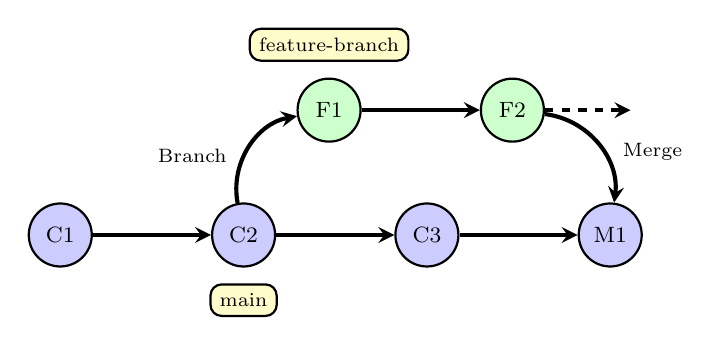
\begin{tikzpicture}[node distance=1.5cm, auto, thick]
    \tikzstyle{commit} = [circle, draw, fill=blue!20, minimum size=0.8cm, font=\footnotesize]
    \tikzstyle{commit_feature} = [circle, draw, fill=green!20, minimum size=0.8cm, font=\footnotesize]
    \tikzstyle{arrow} = [->, >=stealth, line width=1.5pt]
    \tikzstyle{label_box} = [rectangle, draw, fill=yellow!20, rounded corners, font=\scriptsize]

    \node [commit] (c1) {C1};
    \node [commit, right=of c1] (c2) {C2};
    \node [commit, right=of c2] (c3) {C3};
    \node [commit, right=of c3] (m1) {M1};
    
    \node [commit_feature, above right=1cm and 0.5cm of c2] (f1) {F1};
    \node [commit_feature, right=of f1] (f2) {F2};
    
    \draw [arrow] (c1) -- (c2);
    \draw [arrow] (c2) -- (c3);
    \draw [arrow] (c3) -- (m1);
    
    \draw [arrow] (f1) -- (f2);
    
    \draw [arrow] (c2) to [bend left=45] node[near start, above left, font=\scriptsize] {Branch} (f1);
    \draw [arrow] (f2) to [bend left=45] node[near end, above right, font=\scriptsize] {Merge} (m1);
    
    \draw [arrow, dashed] (f2) -- ++(1.5, 0);
    
    \node [label_box, below=0.2cm of c2] {main};
    \node [label_box, above=0.2cm of f1] {feature-branch};
    
\end{tikzpicture}
\end{center}

\par\vspace{0.2cm}
\begin{itemize}
    \item \textbf{Branch}: Create a parallel timeline (\texttt{git checkout -b})
    \item \textbf{Commit}: Work on the feature branch (F1, F2)
    \item \textbf{Merge}: Combine feature history back into main (\texttt{git merge})
    \item \textit{Note: The branch remains open after merging unless deleted}
\end{itemize}
\end{frame}

% Revision item 28; original frame: 24

\begin{frame}[fragile]{Essential Git Commands}
\begin{verbatim}
git status                 # Check current state
git diff                   # Review unstaged edits
git diff --staged          # Review staged edits
git switch -c docs-quickstart  # Create a task branch
git add README.md          # Stage the intended file
git commit -m "Clarify Quick Start"
git log --oneline          # View saved history
git fetch                 # Retrieve remote history
\end{verbatim}
\par\vspace{0.2cm}
\small Inspect local work before switching or integrating branches. Pull behavior depends on configuration. Push and PR creation share work with the remote repository.
\end{frame}

% Revision item 29; original frame: new

\begin{frame}[fragile]{Worktree Commands: One Writer per Folder}
\begin{verbatim}
# From the repository, start at an agreed commit:
git status
git worktree add ../workshop-docs -b docs-quickstart HEAD
git worktree list
# Start the writing agent inside ../workshop-docs
# Give the reviewer the candidate diff and task brief.
\end{verbatim}
\par\vspace{0.2cm}
\begin{itemize}
\item Uncommitted edits are not copied into a new worktree.
\item Use distinct output paths when sessions run concurrently.
\item Preserve and integrate needed work before removing a worktree.
\end{itemize}
\par\vfill
\sources{\href{https://git-scm.com/docs/git-worktree}{Git: worktree}}
\end{frame}

% Revision item 30; original frame: 27

\begin{frame}{Git Best Practices}
\begin{block}{Commit Messages}
\begin{itemize}
\item Be descriptive: ``Clarify README build instructions''
\item Keep each commit focused on one task
\item Link to the relevant issue when there is one
\end{itemize}
\end{block}
\begin{block}{What to Commit}
\begin{itemize}
\item Source code, documentation, and small permitted teaching data
\item Generated outputs only when the project's sharing policy calls for them
\item Keep credentials and restricted data outside the repository
\end{itemize}
\end{block}
\end{frame}

% Revision item 31; original frame: 28

\begin{frame}[fragile]{The .gitignore File}
\begin{columns}[t]
\begin{column}{0.48\textwidth}
\textbf{Example patterns}
\begin{verbatim}
__pycache__/
.venv/
*.aux
*.log
output/
.env
\end{verbatim}
\end{column}
\begin{column}{0.48\textwidth}
\begin{itemize}
\item Applies to untracked files
\item Does not remove a file already tracked
\item Can appear in subdirectories
\item Does not erase secrets from history
\end{itemize}
\end{column}
\end{columns}
\par\vspace{0.3cm}
Inspect \texttt{git status} and the staged diff before committing. An ignore rule helps prevent accidents; it does not enforce data policy.
\end{frame}

% Revision item 32; original frame: 30

\begin{frame}{Resolving Merge Conflicts in VS Code}
\begin{center}
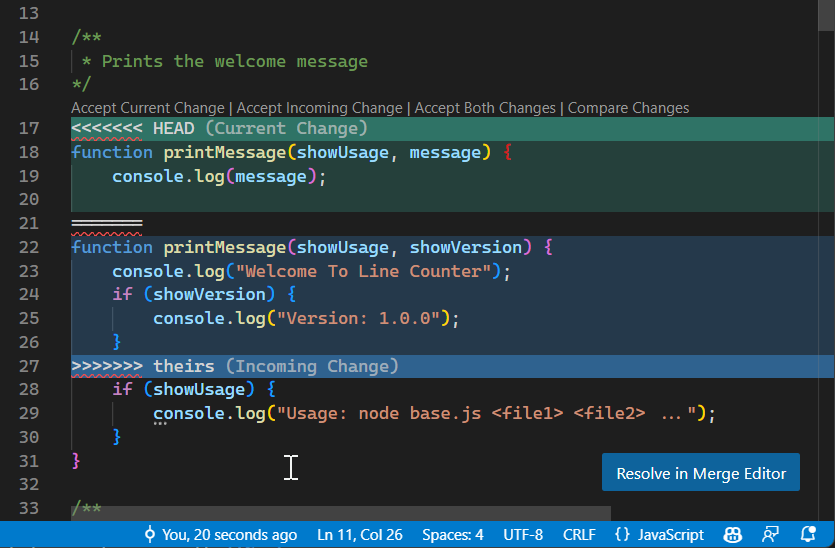
\includegraphics[width=0.45\textwidth,height=3.6cm,keepaspectratio]{figures/merge_conflict.png}
\end{center}

\par\vspace{0.2cm}
\begin{itemize}\setlength{\itemsep}{2pt}
    \item VS Code shows \textbf{conflict markers}: \texttt{<<<<<<< HEAD} (yours) vs \texttt{>>>>>>> theirs}
    \item One-click options: \textit{Accept Current}, \textit{Accept Incoming}, \textit{Accept Both}, or \textit{Compare}
    \item Use \textbf{Resolve in Merge Editor} for a side-by-side 3-way diff
\end{itemize}
\end{frame}

% Revision item 33; original frame: 12

\begin{frame}{Useful VS Code Features}
\begin{columns}[t]
\begin{column}{0.48\textwidth}
\textbf{Navigate and Review}
\begin{itemize}
\item Command Palette: Ctrl/Cmd+Shift+P
\item Quick file open: Ctrl/Cmd+P
\item Search files, symbols, and text
\item Source Control: staged and unstaged diffs
\end{itemize}
\end{column}
\begin{column}{0.48\textwidth}
\textbf{Add What You Need}
\begin{itemize}
\item LaTeX Workshop: source and PDF
\item Python / Jupyter: scripts and notebooks
\item GitHub Pull Requests and Issues
\item Your chosen agent's extension
\end{itemize}
\end{column}
\end{columns}
\par\vspace{0.3cm}
Open the project folder, select the correct environment, and use workspace settings for project-specific tools. Check Keyboard Shortcuts for platform differences.
\end{frame}

% Revision item 34; original frame: 37

\begin{frame}{MCP: Model Context Protocol}
\begin{itemize}\setlength{\itemsep}{0.3cm}
\item MCP connects an agent application to tools and resources exposed by a server.
\item A GitHub connection can expose repository operations, depending on the server and permissions.
\item Native tools and command-line tools are also valid integration paths.
\item Inspect the requested permissions and configure only the access the task needs.
\end{itemize}
\par\vspace{0.3cm}
\textbf{For this workshop:} the instructor can use a prepared connection. Participants do not need to configure MCP for the README exercise.
\par\vfill
\sources{\href{https://modelcontextprotocol.io/docs/learn/architecture}{MCP architecture}; provider setup links in the source notes.}
\end{frame}

% Revision item 35; original frame: 19

\begin{frame}{Data Privacy and Permissions}
\begin{itemize}\setlength{\itemsep}{0.28cm}
\item Use public or permitted teaching material for the exercises.
\item Check institutional policy and the account's terms before providing research data.
\item Local execution does not by itself mean local model inference.
\item Inspect connected tools, network access, and output destinations.
\item Ask before actions outside the task's agreed scope, including publishing or sending messages.
\end{itemize}
\par\vspace{0.25cm}
\small An offline workflow requires checking the whole configuration. A locally installed editor or agent alone does not establish that no data leaves the machine.
\end{frame}

% Revision item 36; original frame: 40

\begin{frame}{Overleaf, Statistical Software, and VS Code}
\begin{block}{Statistical Software}
Use the language extension or terminal workflow supported by your installation. Check paths, licenses, working directories, and the exact command on a small file.
\end{block}
\begin{block}{Overleaf}
Agree where the authoritative draft lives and who synchronizes changes. Check available Git or GitHub integration for the account. Integrate reviewed changes through one owner, then inspect the compiled PDF.
\end{block}
\par\vspace{0.25cm}
Avoid concurrent edits to the same checkout through multiple sync systems. Keep a recoverable copy before synchronizing.
\end{frame}

% Revision item 37; original frame: 47

\begin{frame}[fragile]{The Makefile Approach}
\hypertarget{appendix-makefile}{}
\begin{columns}[t]
\begin{column}{0.48\textwidth}
\textbf{A recipe for the project}
\begin{itemize}
\item Targets declare dependencies and commands
\item Read a target before running it
\item Inspect outputs after a successful build
\end{itemize}
\par\vspace{0.2cm}
\small In this repository, \texttt{make slides} first runs the analysis through \texttt{update-outputs}.
\end{column}
\begin{column}{0.48\textwidth}
\begin{block}{Commands for this revision}
\begin{verbatim}
make help
make slides-only
# Full research workflow:
make all
\end{verbatim}
\end{block}
\small \texttt{slides-only} builds the Beamer deck from the included assets. It does not rerun the analysis.
\end{column}
\end{columns}
\par\vspace{0.4cm}
\hyperlink{main-project-structure}{\beamerbutton{Back to Project Structure}}
\end{frame}

% Revision item 38; original frame: new

% Optional substantive research exercise retained from the original workshop.
\begin{frame}{Research Exercise: Audit the Robustness Check}
\begin{enumerate}\setlength{\itemsep}{0.22cm}
\item Open the existing paper's robustness table and its discussion.
\item Trace the table to \texttt{scripts/analysis.py}: default OLS versus standard errors clustered by \texttt{region\_id}.
\item Ask one agent to check the implementation and another to compare the table with the prose.
\item Require file/line evidence, assumptions about clustering, and a list of claims that need a rerun to verify.
\item Draft a bounded issue and review plan before changing the analysis.
\end{enumerate}
\par\vspace{0.25cm}
\small The original clustered-SE task is already implemented. Audit the existing work, or choose an instructor-approved extension. This optional exercise can replace the README exercise after rehearsal.
\end{frame}

\begin{frame}{VS Code Session Discovery: Scope Matters}
\begin{itemize}\setlength{\itemsep}{0.24cm}
\item Local external Claude Code and Codex sessions can be discovered. They are hidden by default; enable \textit{External} in the sessions-list filter.
\item The setting is \texttt{chat.agentSessions.showExternal}.
\item Codex continuation requires a single writer: fully quit the other application, then retry in VS Code.
\item The OpenAI extension and experimental Codex Agent Host are distinct integration surfaces.
\end{itemize}
\par\vspace{0.25cm}
\small Remote SSH/tmux session discovery is not established by the local-session documentation. Rehearse the exact setup before promising it in a demo.
\par\vfill
\sources{\href{https://code.visualstudio.com/docs/agents/run/sessions/manage-sessions}{Manage sessions}; \href{https://code.visualstudio.com/docs/agents/run/agent-harnesses}{agent harnesses}.}
\end{frame}

% Revision item 39; original frame: 44

\begin{frame}{Resources}
\begin{columns}[t]
\begin{column}{0.48\textwidth}
\textbf{Project Workflow}
\begin{itemize}
\item \href{https://git-scm.com/doc}{Git documentation}
\item \href{https://docs.github.com}{GitHub documentation}
\item \href{https://code.visualstudio.com/docs}{VS Code documentation}
\item \href{https://skills.github.com}{GitHub Skills}
\end{itemize}
\end{column}
\begin{column}{0.48\textwidth}
\textbf{Agent Documentation}
\begin{itemize}
\item \href{https://code.claude.com/docs}{Claude Code}
\item \href{https://developers.openai.com/codex}{Codex}
\item \href{https://modelcontextprotocol.io/docs}{Model Context Protocol}
\item \href{https://github.com/tlarroucau/AI_workshop}{Workshop repository}
\end{itemize}
\end{column}
\end{columns}
\par\vspace{0.4cm}
\small Product availability depends on version, surface, account, and organization settings. The accompanying source notes record the documentation used for this revision.
\end{frame}

\end{document}
